\section{Incrementally maintain classifiers}
%road map
In this section, some recent works on incrementally maintaining materialized classifier parameters in database are presented, which initially originates from \cite{deshpande2006mauvedb} and follows by \cite{koc2011incrementally}. Both \cite{deshpande2006mauvedb} and \cite{koc2011incrementally} develop a system (MauveDB vs Hazy) to store typical statistical model parameters as database view in RDBMS and update the views incrementally when raw data are modified.   

\subsection{MauveDB}
%brief description to MauveDB
MauveDB primarily deals with wireless sensor network applications, where data are collected through underlying sensors, fitted with typical statistic model such as regression-based model and interpolation-based model and used for estimating missing or future results. The statistic models learned with those raw data are materialized as {\em model-based views}, which are created with a high-level SQL-like language. Due to the addition or removal of the sensors, raw data are updated constantly, which requires efficient view maintenance strategies. The details of how {\em model-based views} are defined, updated and queried for prediction are provided as follows, which highly depend on the types of statistical model.

\subsubsection{Basic notations}
We will use capitalized letters (e.g. $H$) to denote matrix, capitalized bold letters (e.g. $\textbf{T}$) to denote tables, lowercase letters (e.g. $x$ and $y$) to denote scalar value, bold lowercase letters (e.g. $\textbf{x}$) to denote variables, lowercase letters with bar (e.g. $\bar{w}$) to denote a vector, $f(*)$ to denote functions ($*$ represents arguments of function $f$). Besides, we use $H_{i,j}$ to denote the value at cell $(i,j)$ in matrix $H$ and use $\bar{w}_i$ to denote $i_{th}$ element in vector $\bar{w}$. We introduce superscript $^{(t)}$ (e.g. $x^{(t)}$) to denote the value of certain variables at the time step $t$ during iterative computation. Based on those notations, we provide notations for each model as follows.

\paragraph{Regression model}
A regression model is usually written as the following form:
\begin{equation}
t=\sum_{i=1}^kw_ih_i(*)
\end{equation}
where $h_i$ represents {\em basis function}, which is a monomial of {\em predictor variables} while $w_i$ represents coefficient of those monomials and $t$ is the {\em response variable}.

For example, in wireless sensor network application, temperature is measured at a 2D-space with coordinate $x$ and $y$, which can be computed with the following typical polynomial of the two predicator variables:

\begin{equation}
temp=w_1 + w_2x+w_3x^2 + w_4y+w_5y^2
\end{equation}
where the basis functions are $\{h_1(x,y), h_2(x,y), h_3(x,y),h_4(x,y), h_5(x,y)\}=\{1, x, x^2, y, y^2\}$

Given a set of data observed from the underlying wireless sensors located at different positions, $\{x_j,y_j,temp_j\}(j=1,2,\dots,n)$, the coefficients $\bar{w}^* = \{w_1,w_2,\dots,w_k\}$ are estimated with the following linear system:
\begin{equation}\label{eq: regression_solve}
    H^TH\bar{w}^*=H^T\bar{f}
\end{equation}

where $H$ is:
\begin{equation}
    H=\begin{bmatrix}
h_1(x_1,y_1) & h_2(x_1,y_1) &\dots &h_k(x_1,y_1)\\
h_1(x_2,y_2) & h_2(x_2,y_2) &\dots &h_k(x_2,y_2)\\
\dots\\
h_1(x_n,y_n) & h_2(x_n,y_n) &\dots &h_k(x_n,y_n)
\end{bmatrix}
\end{equation}

and $\bar{f}$ is:

\begin{equation}
    \bar{f} = \{temp_1, temp_2,\dots, temp_n\}^T
\end{equation}

In general, $H$ will be a matrix which represents data sets of $n$ data points with $k$ features while $\bar{f}$ represents the label vectors.

\paragraph{Interpolation model} 

The goal of interpolation is to estimate missing values of response variables given a value of predictor variable, which does not exist in the set of existing value pair for predictor variable and response variable. Specifically, given a variable pair $(\textbf{t},\textbf{v})$ and a set of value pairs for those two variables, $(t_i, v_i)(i=1,2,\dots,n)$ observed from sensors are then used to estimate value $v'$ of variable $V$ given a value $t'$ of variable $T$ $(t_j< t' < t_{j+1})$. Usually, {\em linear interpolation} is used. So $v'$ is estimated with value pair $(t_j, v_j)$ and $(t_{j+1}, v_{j+1})$ as follows:
\begin{equation}\label{eq: interpolation}
    v'= v_j + (v_{j+1}-v_j)\times\frac{t'-t_j}{t_{j+1}-t_j}
\end{equation}




\subsubsection{View definition}

MauveDB developed an declarative SQL-like language for users to define model-based view, which is exemplified in Figure \ref{fig:MauveDB_view_def}. Although different models cannot be manipulated in exactly the same way due to their different characteristics, the commonalities are still leveraged in this language. 

In Figure \ref{fig:MauveDB_view_def}, examples of regression-based view and Interpolation-based view definitions are presented in (i) and (ii) respectively. Same as way to create other database views, the view schemas, where the raw data comes from to construct the views (represented by \textit{SELECT}, \textit{FROM}) and what conditions the raw data should satisfy (represented by \textit{WHERE}) should be declared in the view definition statements. The model types (\textit{FIT} and \textit{INTERPOLATE} for regression and interpolation respectively) should be also specified along with partitions of raw data on each of which the models are trained (\textit{FOR EACH}) and other model-related information (such as base function for regression model, represented by \textit{BASE}). After executing statements shown in Figure \ref{fig:MauveDB_view_def}, {\em model-based views} are then created and stored in the RDBMS as relational tables.


\begin{figure}
    \centering
    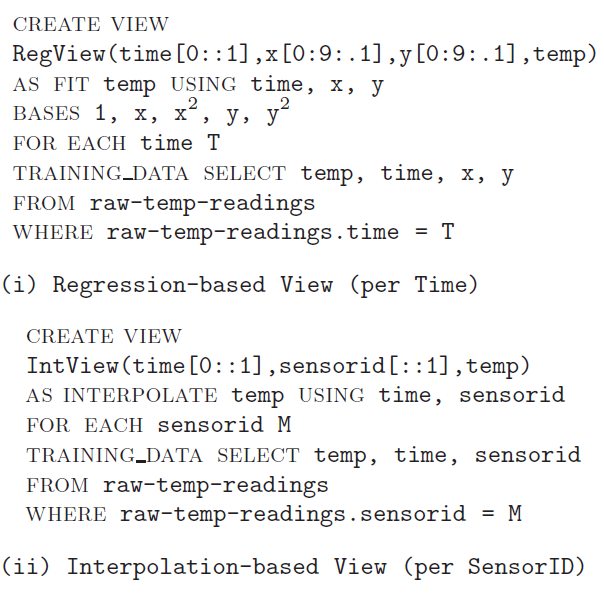
\includegraphics[width=8cm, height=8cm]{Figures/MauveDB_create_view.png}
    \caption{Define views in MauveDB}
    \label{fig:MauveDB_view_def}
\end{figure}

\subsubsection{View maintenance}
%High-level descriptions of view maintenance strategies
When the new data are available, the updates should be reflected on the model-based views. Four different strategies are developed for this purpose and their trade-offs are discussed with extensive experiments. The details of the four view maintenance strategies are introduced in this section.

\textit{Strategy 1: Materialize the views (eager approach)}
A naive way is simply to construct the models and materialize the model parameters as views in the database, which can avoid unnecessary query execution time when users want to retrieve the ``exact'' model information. However, such views may incur high space overhead and pose a challenge in refreshing the model as new data comes.

\textit{Strategy 2: Always use the base data }
This strategy goes to another extreme without materialization at all in the database, which can obviously make query processing very expensive since recomputating the view content is necessary every time when queries are evaluated. 

\textit{Strategy 3: Partial materialization (lazy approach)}
Somewhere in-between is to partially materialize the view content, which simply caches parts of the views that have been computed by certain queries. When the views are about to be refreshed, the corresponding cached contents in memory will be invalidated.

\textit{Strategy 4: Materialize an intermediate representation}
Some intermediate representations are materialized in this strategy by leveraging some nice properties of regression model and interpolation model, which have been an efficient solution experimentally and are presented as follows for the two models respectively.

For regression model, recall that the optimal coefficients can be solved with Equation \ref{eq: regression_solve}. The intermediate representation for it can be simply the materialization of matrix $H^TH$ and $H^T\bar{f}$, which can be beneficial in various aspects. First, the dimensions of the two matrices only rely on the total number of features, which thus won't lead to large space overhead. Besides, efficient updates to the two matrices are achievable since they are computed with linear operators, i.e. matrix multiplications and additions. A newly generated data point $(x',y', temp')$ can trigger the update of $H^TH$ and $H^T\bar{f}$ as follows:
\begin{equation}
    (H^TH)^{new}_{i,j} = (H^TH)^{old}_{i,j} + h_i(x',y')*h_j(x',y')
\end{equation}
\begin{equation}
    (H^T\bar{f})^{new}_i = (H^T\bar{f})^{old}_i + h_i(x',y')*temp'
\end{equation}

Once the user queries arrive, the coefficient $\bar{w}$ is computed with the following expression:
\begin{equation}
    \bar{w}^*=(H^TH)^{-1}H^T\bar{f}
\end{equation}

which can be computed with time complexity $Q(k^3)$ where $k$ is the total number of features.

For interpolation model, following the example shown in Figure \ref{fig:MauveDB_view_def}, the data in the interpolation-based view $\textbf{V}$ will be of the form $(\textbf{t}, \textbf{v})$ where $\textbf{t}$ represents time while $\textbf{v}$ represents observed value by the sensors. Unlike regression mode, its intermediate representations are not additional data but some additional data structure for searching the values of variable $\textbf{t}$. In order to efficiently estimate the sensor values for time $t'$ which is missing from the view instance but queried by users, the closest values $t_{-}$ and $t_{+}$ (along with the corresponding sensor values $v_{-}$ and $v_{+}$) to $t'$ are retrieved with the auxillary data structure such that $t'$ lies in the interval $(t_{-}, t_{+})$ with no other $\textbf{t}$ value from $\textbf{V}$ in it. So the estimated sensor value at time $t'$ can be computed using Equation \ref{eq: interpolation}.

The specific choice of strategies in practice depends on various factors, such as the query workload, data statistics and types of models. The trade-off between the four strategies are experimentally explored with extensive experiments in \cite{deshpande2006mauvedb}, which shows that the strategy 4 performs best in most scenarios while strategy 1 can actually outperform others in some cases.

\subsection{Hazy}
Hazy is another system for incrementally maintaining classifiers in RDBMS, which extends and improves MauveDB in the following aspects. 1) more linear classifers are supported, including support vector machines, ridge regression and logistic regression; 2) both eager and lazy strategies used in MauveDB are optimized by speeding up the updates and read operations.

\subsubsection{Views in Hazy}
\begin{figure}
    \centering
    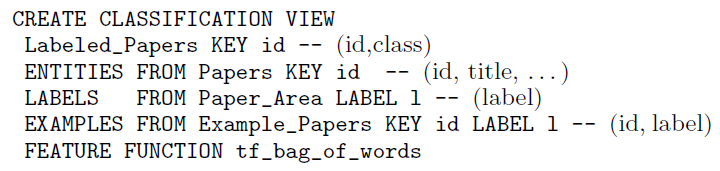
\includegraphics[width=10cm, height=2.5cm]{Figures/Hazy_view.png}
    \caption{Define views in Hazy}
    \label{fig:Hazy_view_def}
\end{figure}

%intro to view definition
In Hazy, users can declare views in the way shown in Figure \ref{fig:Hazy_view_def}, in which a {\em classification view} is defined over some entity table (i.e. $Papers$ in Figure \ref{fig:Hazy_view_def}, with Primary key $id$) to identify their type (i.e. $Paper\_area$) with a model trained using some training examples (i.e. $Examples\_papers$) that are derived from original entity table by applying some feature function (i.e. $tf\_bag\_of\_words$ function). So in the end, the content of the classification view is the classification results for the set of entities to be classified, in which each tuple has the form $(id, class)$ where $id$ is the entity id while $class$ is the label for that entity determined by the model. The major difference between eager and lazy strategies in terms of classification view definition is that the former one stores the materialized views in the database while the latter one only keeps views virtual.

%operations in Hazy and the bottleneck for eager and lazy approach
Hazy focus on three typical queries issued by the users: 1) {\em Single entity} read, i.e. retrieve the label of a single entity; 2) {\em All members} read, i.e. retrieve the labels for all the entities; 3) {\em Update}, i.e. update the views once new training examples arrive. Intuitively, the {\em update} should become the bottleneck for eager approach since the materialized views should be refreshed whenever updates happen while the {\em All members} read should be the major overhead for lazy approach since the content of the virtual views should be computed whenever read queries are issued, which are the major concerns for the authors of Hazy. In terms of {\em update} queries, the authors of Hazy assume that in the time to retraining the model is negligible (roughly on the order of 100$\mu$s on their datasets) and the major overhead is to relabel the entities in the materialized views for eager approach. 

\subsubsection{Overview of view maintenance in Hazy (eager approach)}
%overview of view maintenance problem
In this section, the details on how to maintain materialized classification views in Hazy are provided, which targets at more efficient {\em update} queries for eager approach rather than recomputing the content of views from the scratch when updates arrive. Lazy approach is free from this issue since updates won't influence the virtual views in the database. 

%introduce notation for table H
Suppose support vector machine is used thereafter (more complicated classifiers are introduce later) for binary classifications, at epoch $i$, the model parameters will be $(\bar{w^{(i)}}, b^{(i)})$. Given an entity with feature vector $\bar{f}$, its label is determined by the sign of the residual $eps = \bar{w^{(i)}}*\bar{f}-b^{(i)}$. If $eps > 0$ ($eps < 0$ respectively), then this entity is labeled as $+$ ($-$ respectively).

Recall the assumption that the time to retrain the model is not significant, the model is firstly retrained at each epoch. Given the updated model parameters, a scratch table $\textbf{H}$ is maintained inside Hazy and varied across different epochs, which stores tuples of the form $(id, \bar{f}, eps)$ where $id$, $\bar{f}$ and $eps$ represents the entity id, feature vector and residual ($eps = \bar{w^{(i)}}*\bar{f}-b^{(i)}$). Then the classification view $\textbf{V}$ can be obtained from $\textbf{H}$, in which each view tuple has the form $(id, c, eps)$ ($c$ is the label for entity with identifier $id$ and is calculated as $c=sign(eps)$). For a tuple $t \in \textbf{H}$ ($\in \textbf{V}$), we use $t.attr$ denote the value of attribute $attr$ at tuple $t$ where $attr$ is an attribute of $\textbf{H}$ ($\textbf{V}$ respectively). For example, $t.\bar{f}$ and $t.id$ represent the feature vector and the entity at tuple $t$ in $\textbf{H}$.

%introduce two steps
\paragraph{Incremental step VS reorganization step} At epoch $i$, Hazy maintains table $\textbf{H}^{(s)}$ which is constructed at epoch $s$ ($s < i$), view $V^{(i+1)}$ can be either {\em incrementally} constructed from $V^{(i)}$ by updating small portion of view tuples in $V^{(i)}$ without changing $\textbf{H}^{(s)}$ or computed by referencing latest $\textbf{H}$ ({\em reorganized} at epoch $i$). Intuitively, the {\em incremental} step is relatively cheaper since it only touches parts of the view content, which, however, can incur more overhead when the model is far away from the model in the beginning as the time goes by. So the {\em reorganization step} is needed after applying the {\em incremental step} for some epochs to reduce the overhead in the following epochs to apply {\em incremental step}.

%cost of the two options
\paragraph{Cost measure and skiing strategy} In order to determine the optimal strategy on which step to take at each epoch, Hazy quantifies the cost for each of the two steps and formalizes it as the classic {\em ski rental problem}. In this problem, the cost of the {\em incremental option} is defined as the time to update $V^{(i)}$ to $V^{(i+1)}$, which should be proportional to the view tuples relabeled at epoch $i$ (denoted as $c^{(i)}$) while the {\em reorganization step} has a fixed cost $S$. Suppose the {\em reorganization step} is taken at epoch $s$, then the accumulated cost at epoch $i$ by applying {\em incremental step} since epoch $s$ is $a^{(i)} = \sum_{j=s+1}^ic^{(j)}$. The strategy to choose proper steps ({\em skiing strategy}) is as follows: If the accumulated cost $a^{(i)}$ is too large, say, greater than $\alpha S$ ($\alpha$ is a constant), then refreshing table $H$ is needed (the accumulated cost $a^{(i)}$ is reset to 0 after that). This strategy is proven to be 2-approximation asymptotically compared to the optimal strategy.


\subsubsection{Details of incremental step}\label{Sec: incremental step}
%overview
The core idea of {\em incremental step} is to do small changes to the classification view content to reflect the updates approximately, the details of which are presented as below. It starts by introducing how to determine which part of view tuples to be changed at each epoch with two thresholds, which follows by the detailed derivation rules of the two thresholds.

\paragraph{Thresholds in incremental step}
%intro to lower water and higher water
For incremental step, it is assumed that the appearance of the new training examples do not result in great changes to the model, which means that it is safe to simply update small portion of the view content to achieve performance gains at each epoch. Intuitively, the entities that are far away from the decision boundary should be less likely to be changed when the updates happen while the ones closer to the decision boundary are more likely to flip the labels. So Hazy introduces two thresholds, lower water and higher water (denoted by $lw$ and $hw$ respectively, which are negative and positive respectively) to determine which view tuples should be changed or not. At each epoch $i$, by referencing the residual value $eps$ for each entity in the scratch table $\textbf{H}^{(s)}$ computed at epoch $s$ ($s<i$), if $eps$ is greater than $hw$ (less than $lw$), then the labels of the corresponding entities are (highly likely to be) $+$ ($-$ respectively) and thus remain unchanged. Otherwise, we use the updated model at epoch $i$ to reclassify those entities. 

%how to compute lower water and higher water
\paragraph{How to determine the thresholds}
Intuitively, the two thresholds $hw$ and $lw$ should be adjusted at each epoch $i$ since the differences between model at epoch $i$ and model at epoch $s$ (when $\textbf{H}$ is recomputed) may be varied for different $i$. So $hw$ and $lw$ are associated with superscript $^{(s,i)}$ to indicate that they are related to the models at epoch $s$ and $i$, i.e. $hw^{(s,i)}$ and $lw^{(s,i)}$ respectively, which are computed as follows:

\begin{equation}
    lw^{(s,i)} = min_{l=s,\dots, i}\epsilon_{low}^{(s,l)},
    hw^{(s,i)} = min_{l=s,\dots, i}\epsilon_{high}^{(s,l)}
\end{equation}

where $\epsilon_{low}^{(s,l)}$ and $\epsilon_{high}^{(s,l)}$ are computed as (recall that $t.\bar{f}$ represents the feature vector of $t$):
\begin{equation}
    \epsilon_{low}^{(s,l)} = max_{t \in \textbf{H}}||t.f||_q||\bar{w^{(s)}}-\bar{w^{(l)}}||_p+b^{(s)}-b^{(l)}, \epsilon_{high}^{(s,l)} = - max_{t \in \textbf{H}}||t.f||_q||\bar{w^{(s)}}-\bar{w^{(l)}}||_p+b^{(s)}-b^{(l)}
\end{equation}
where the norm $q$ and $p$ satisfy $p^{-1} + q^{-1} = 1$


There is a nice property by applying Holder's inequality \cite{rudin1976principles} to $\epsilon_{low}^{(s,j)}$ and $\epsilon_{low}^{(s,j)}$, i.e. at epoch $j$, for a tuple $t \in \textbf{H}^{(s)}$, if $t.eps \geq \epsilon_{high}^{(s,j)}$ ($t.eps \leq \epsilon_{low}^{(s,j)}$), then $t.id$ should be in the class $+$ ($-$).

\subsubsection{Details of reorganization step}
The {\em reorganization step} for the scratch table $\textbf{H}$ includes recomputing the residual $\epsilon$ for each entity in $\textbf{H}$, reconstructing necessary indexes to quickly search the entity in $\textbf{H}$ and sorting the entire table by the residual $eps$, which happens when the current model is far away from the model computed in the last reorganization step. A greedy strategy is proposed earlier.  Formally speaking, when the cost of {\em reorganization step} (fixed as $S$, which is the time to perform the {\em reorganization step}) is less than the accumulated cost $a_{i}$, {\em reorganization step} is executed.

\subsubsection{Analysis of the greedy strategy}
Two assumptions about the cost measure are made when designing such greedy strategy: 1) the cost of incremental step, $c^{(s, i)}$ only depends on the current epoch $i$ and the most recent epoch $s$ for reorganization step since $c^{(s, i)}$ is a function of the number of tuples within the interval $[lw^{(s,i)}, hw^{(s,i)}]$; 2) Reorganization more recently won't increase the cost $c^{s,i}$, which means that $c^{(s, i)} < c^{(s',i)}$ for $s > s'$. The assumptions above can guarantee 2-approximation compared to theoretical optimal strategy. The analysis is sketched as follows.

%notations
Suppose during reorganization step, it takes $\sigma S$ to scan $\textbf{H}$. Given $N$ epochs in total, reorganization step is executed $M$ times, which happens at epoch $\mu_1, \mu_2,\dots, \mu_M$ ($0 \leq \mu_1 < \mu_2 < \dots < \mu_M \leq N$), The integer sequence $\bar{\mu} = \mu_1, \mu_2,\dots, \mu_M$is defined as a {\em schedule} under a certain strategy. At any epoch $i$, we define $\floor{i}_{\bar{\mu}} = max\{\mu \in \bar{\mu} | \mu < i\}$, which intuitively returns the most recent epoch before epoch $i$ when {\em reorganization step} is executed. Denote the set of costs for every epoch by $\bar{c} = \{c^{(s,i)}\}$, the total cost of a {\em schedule} will be:
\begin{equation}\label{eq: cost}
    Cost(\bar{\mu}, S, \bar{c}) = \sum_{i=1,2,\dots,N}c^{(\floor{i}_{\bar{\mu}}, i)} + MS
\end{equation}

Equation \ref{eq: cost} indicates that the total cost not only depends on how to schedule the reorganization step, but also depends on the cost at each epoch, i.e., $\bar{c}$ and $S$. This is because at each epoch, the value of $c^{(\floor{i}_{\bar{\mu}}, i)}$ is known to us only after the incremental step is over (recall that $c^{(s,i)}$ represents the execution time of incremental step), which can influence the accumulated cost $a^{(i)}$ and thus influence the decision at some point (recall that the decision at epoch $i$ depends on whether $a^{(i)}$ is greater than $\alpha S$). So given a strategy $\Phi$, the schedule $\bar{\mu}$ should be a function of $\bar{c}$, i.e. $\bar{\mu} = \Phi(\bar{c})$.

In order to prove that the skiing strategy is a 2-approximation strategy, the {\em competitive ratio} (denoted by $\rho$) is defined as below, which is a ratio between the cost of a strategy $\Phi$ and and the optimal cost:
\begin{equation}
    \rho(\Phi) = sup_{\bar{c}}\frac{Cost(\bar{\mu}, S, \bar{c})}{Cost(\bar{o}, S, \bar{c})}
\end{equation}


It is proven that $\rho(skiing) = (1+\alpha + \sigma)$ where $\alpha$ is the positive root of $x^2 + \alpha x - 1$ and for any other deterministic strategy, $\rho(\Phi) \geq (1+\alpha + \sigma)$. Specifically, when the number of entities goes to infinity, the time to scan $\textbf{H}$ table, i.e. $\sigma S$ should be approaching 0 (recall that $S$ is the reorganization time, which includes the time to sort $\text{H}$. The sorting time is more expensive than scanning time). In this case, $\alpha \rightarrow 1$ and thus $\rho(skiing) \rightarrow 2$.

\subsubsection{Overview of read queries in Hazy (lazy approach)}
%overview
In this section, how Hazy improves the performance on read queries, i.e. {\em single entity} read and {\em all members} read is presented. Recall that in eager approach, the classification views are materialized. So read queries are not a bottleneck here since the labels of either single entity or all the entities can be retrieved from the view instance directly. On contrast, only the virtual views are used in lazy approach, which may slow down the read queries since the view content should be generated on line. As a result, the authors focus on improve the performance of read queries (especially {\em all members} queries) for lazy approach.

Suppose a user wants to retrieve all the entities of the positive class, which is a typical {\em all members} query, in the naive solution, at a certain epoch $i$, all the entities need to be scanned to be labeled with the current model. However, in Hazy, not all the entities are read to respond to this query, which are achieved by referencing the scratch table $\textbf{H}^{(s)}$ (reorganized at epoch $s$, $s < i$), reading all the tuple $t$ satisfying $t.eps > lw^{(s,i)}$ from $\textbf{H}^{(s)}$ and simply labeling the entities satisfying $t.eps \in [lw^{(s,i)}, hw^{(s,i)}]$ (recall that entities with residual $t.eps > hw^{(s,i)}$ should be guaranteed to be in the positive class). 

Same as view maintenance problem in the last few sections for eager approach, there also exists a trade-off on whether the scratch table $\textbf{H}$ should be reorganized. For the read queries for the lazy approach, the greedy strategy is applied to determine when to do reorganization but with different cost measure to quantify the overhead of {\em incremental step}. Suppose it takes $S'$ seconds to read the entire entities, the number of real positive entities is $N_{+}$ and the number of entities above the low water $lw^{(s,i)}$ is $N_{R}$, then the cost of {\em all members} queries will be $c^{(i)} = \frac{N_{R}-N_{+}}{N_{R}}S$ and the accumulated cost is calculated as in Section \ref{Sec: incremental step}. Then the rest of the skiing strategy here is identical to the one used for eager approach.


\subsubsection{Other optimizations in Hazy}
Hazy also provides two types of system variants to achieve the performance enhancement. The first variant of Hazy is to maintain the classification views and the scratch table $\textbf{H}$ in memory (refered as Hazy-MM), which can be safely discarded when reorganizations happen since the model parameters will be recomputed at each epoch. The other one is to hybrid the main-memory structure and the on-disk structure to reduce the memory footprint. The performance trade-offs between the original system design and the two variants are explored experimentally.

\subsubsection{Extends to other machine learning models}
In the previous sections, it is assumed that the default machine learning algorithm is support vector machine. But Hazy is also flexible to handle other machine learning models. 

\subsection{Discussion}


\section{Incrementally compute matrix programs}


\section{Incrementally derive new models with existing models}